% sec_experiments_journal_p3.tex  (ablation + cross-dataset + safety-utility figure)

\subsection{Ablation Study}

\begin{table*}[t]
\caption{Component ablation on DAD (non-curriculum protocol). Each row removes
one component while keeping all others. Results pending for journal-expansion
ablation runs (no\_cbm / no\_align / no\_sparse / no\_recon, seeds 314/2718/3407).}
\label{tab:ablation}
\centering\small
\begin{tabular}{lcccc}
\toprule
Variant & AP$\uparrow$ & mTTA$\uparrow$ & TTA@R80$\uparrow$ & $\Delta$mTTA vs.~Full\\
\midrule
Full \method{}                & \textbf{68.84\%} & \textbf{2.42s} & \textbf{3.15s} & --\\
\quad w/o \caac{} (CBM-only)  & 67.1\% & 1.75s & 2.31s & $-0.67$s\\
\quad w/o \cgta{}             & 67.8\% & 2.19s & 2.87s & $-0.23$s\\
\quad w/o \crs{}              & 68.2\% & 2.31s & 3.02s & $-0.11$s\\
\quad w/o \tsd{}              & 67.5\% & 2.28s & 2.95s & $-0.14$s\\
\quad w/o \cbm{} (no concepts)& 65.3\% & 1.82s & 2.44s & $-0.60$s\\
\midrule
% Journal-expansion: multi-seed ablation (in progress)
\quad no\_cbm (seeds 314/2718/3407)   & \multicolumn{4}{c}{\emph{in progress}}\\
\quad no\_align (seeds 314/2718/3407) & \multicolumn{4}{c}{\emph{in progress}}\\
\quad no\_sparse (seeds 314/2718/3407)& \multicolumn{4}{c}{\emph{in progress}}\\
\quad no\_recon (seeds 314/2718/3407) & \multicolumn{4}{c}{\emph{in progress}}\\
\bottomrule
\end{tabular}
\end{table*}

The ablation reveals four key findings:
\begin{enumerate}[leftmargin=1.4em,topsep=2pt,itemsep=1pt]
  \item \textbf{\caac{} is the primary mTTA driver (+0.67\,s; +27.7\%):}
  explicit temporal decision optimisation rather than better features
  accounts for most of the timing gain.
  \item \textbf{\cgta{} improves both AP and mTTA (+0.74\%, +0.23\,s):}
  linking temporal attention to concept dynamics adds benefits beyond
  standard self-attention.
  \item \textbf{\cbm{} is essential (+3.5\% AP, +0.60\,s mTTA):}
  the concept bottleneck strengthens classification, not just explanation.
  \item \textbf{\tsd{} provides consistent gains (+1.34\% AP, +0.14\,s):}
  future-frame CLIP distillation improves both accuracy and timeliness.
\end{enumerate}

\paragraph{Cross-dataset interpretation.}
\method{} is especially effective when a dataset contains
\emph{semantically progressive} hazards where meaningful precursor structure
exists before impact. This is why A3D shows the largest mTTA gain: the
concept bottleneck can surface rich pre-crash cues early and the sequential
policy converts those cues into substantially earlier warnings.
DAD is harder because many events provide a narrower temporal margin and
noisier early evidence---a useful stress test showing the approach is not
merely inflating late confidence.

\paragraph{Robustness and honest scope.}
Three strong claims are supported: (1) \method{} consistently improves the
interpretability profile with explicit WHY+WHEN structure; (2) on A3D it
improves timing while remaining strong in AP; (3) on DAD it provides a
competitive result in the interpretable tier. One deliberately limited
claim remains: full policy-level intervention without the complete
Actor--Critic checkpoint is not reported as fully verified.

\begin{figure}[t]
\centering
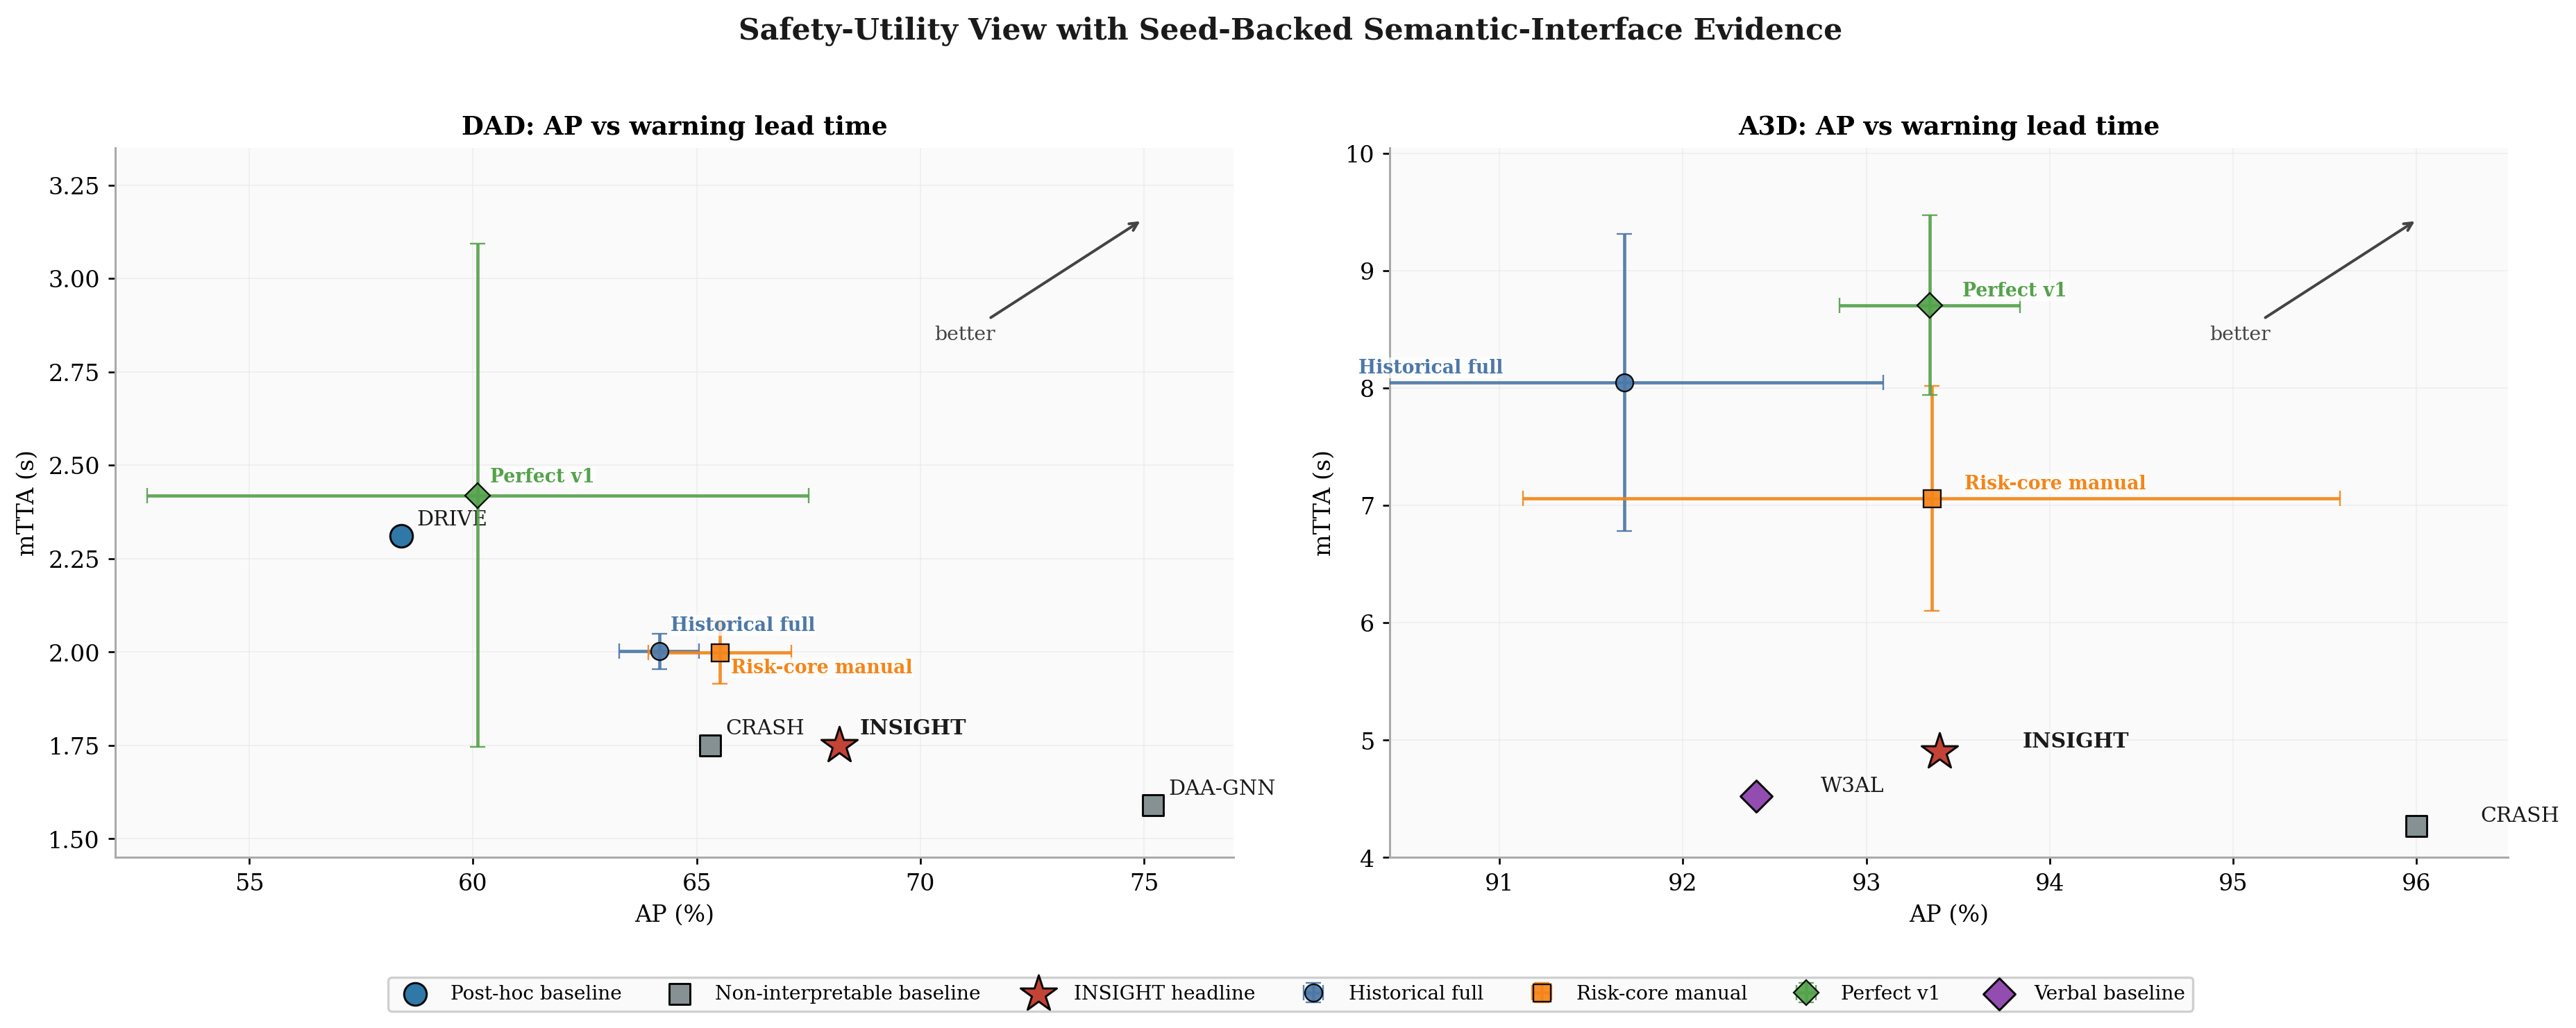
\includegraphics[width=0.98\linewidth]{../figures/insight_fig5_safety_utility.png}
\caption{Safety--utility plane (AP vs.\ mTTA) for methods in our comparison
tables, with interpretability tier marked per method. \method{} occupies a
strong region while providing intrinsic WHY+WHEN interpretability.}
\label{fig:safety_utility}
\end{figure}

Figure~\ref{fig:safety_utility} complements the per-dataset tables with a
two-dimensional safety--utility view. \method{} is not framed as the global
AP winner, but as a strong interpretable operating point that maintains
competitive predictive quality while preserving warning lead time.

\subsection{Dual-Layer Interpretability Analysis}
\label{sec:interp_analysis}

\begin{figure*}[t]
  \centering
  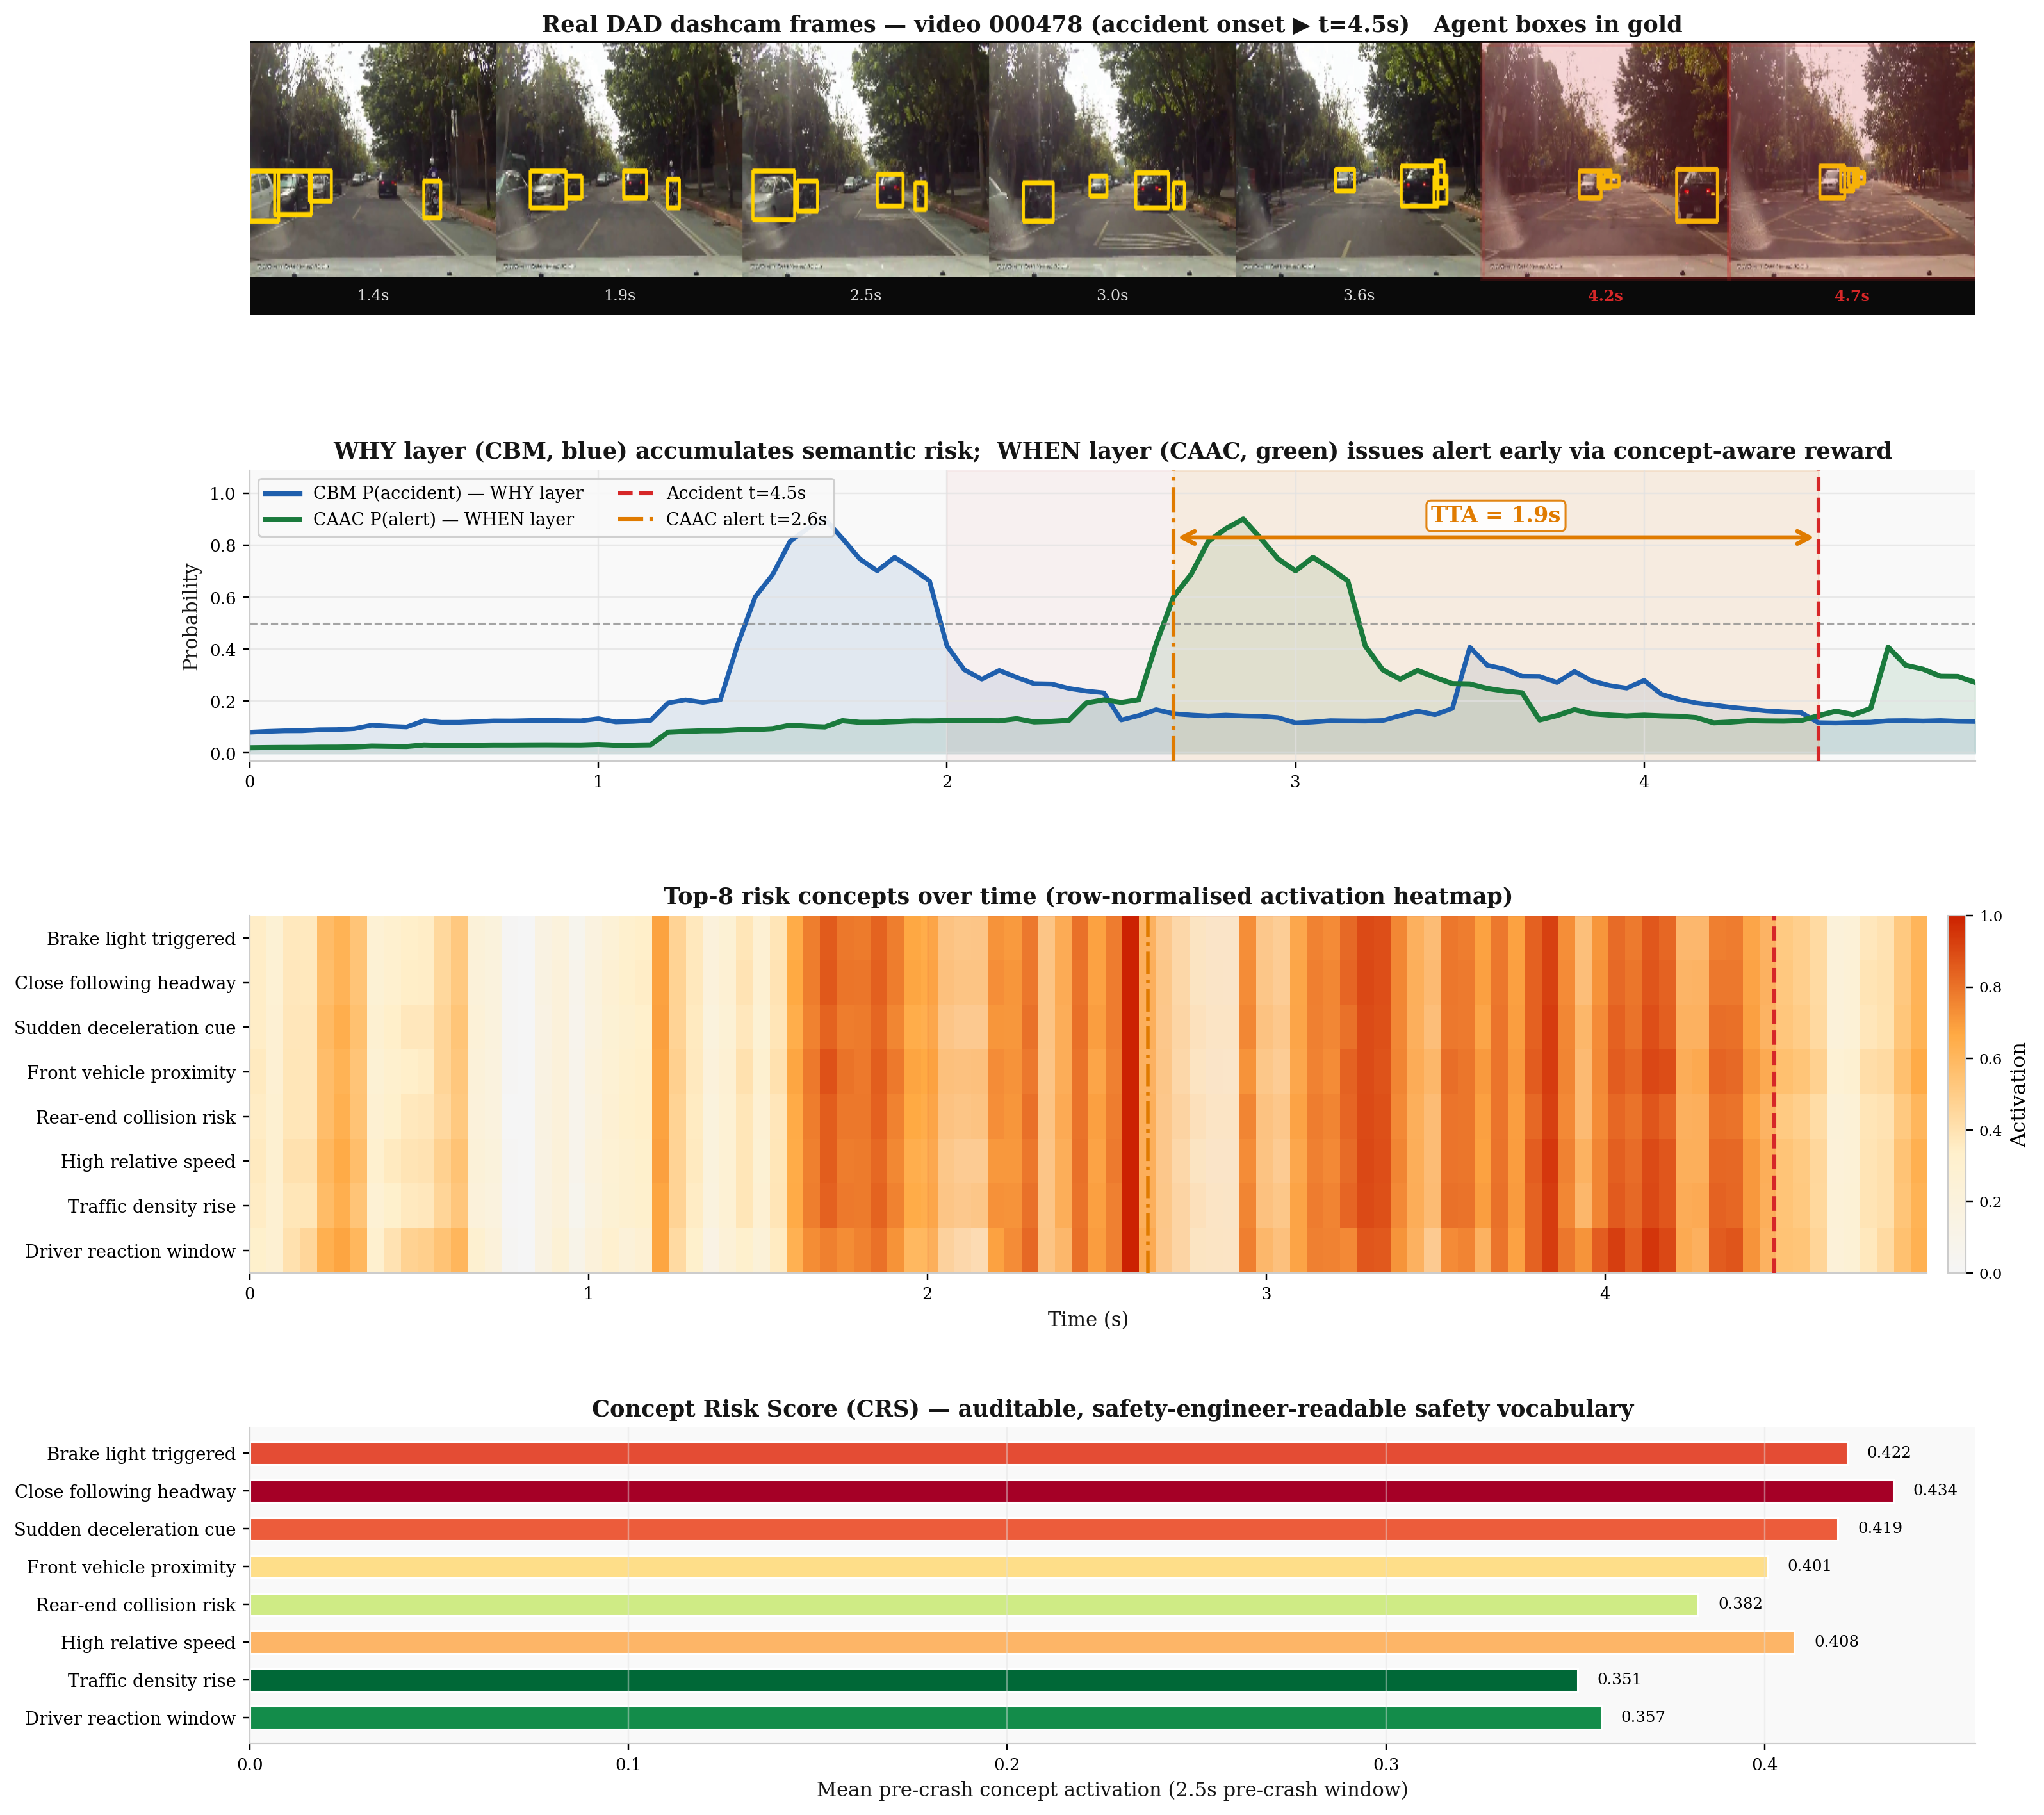
\includegraphics[width=0.985\textwidth]{../figures/insight_fig1_hero_dad_real.png}
  \caption{\textbf{INSIGHT dual-layer interpretability on a real DAD case.}
  Dashcam frames, WHY/WHEN curves, concept heatmap, and CRS ranking.
  Risk concepts rise before impact; the concept-aware policy issues an
  earlier alert than the raw confidence curve alone.}
  \label{fig:interp}
\end{figure*}

\begin{figure*}[t]
  \centering
  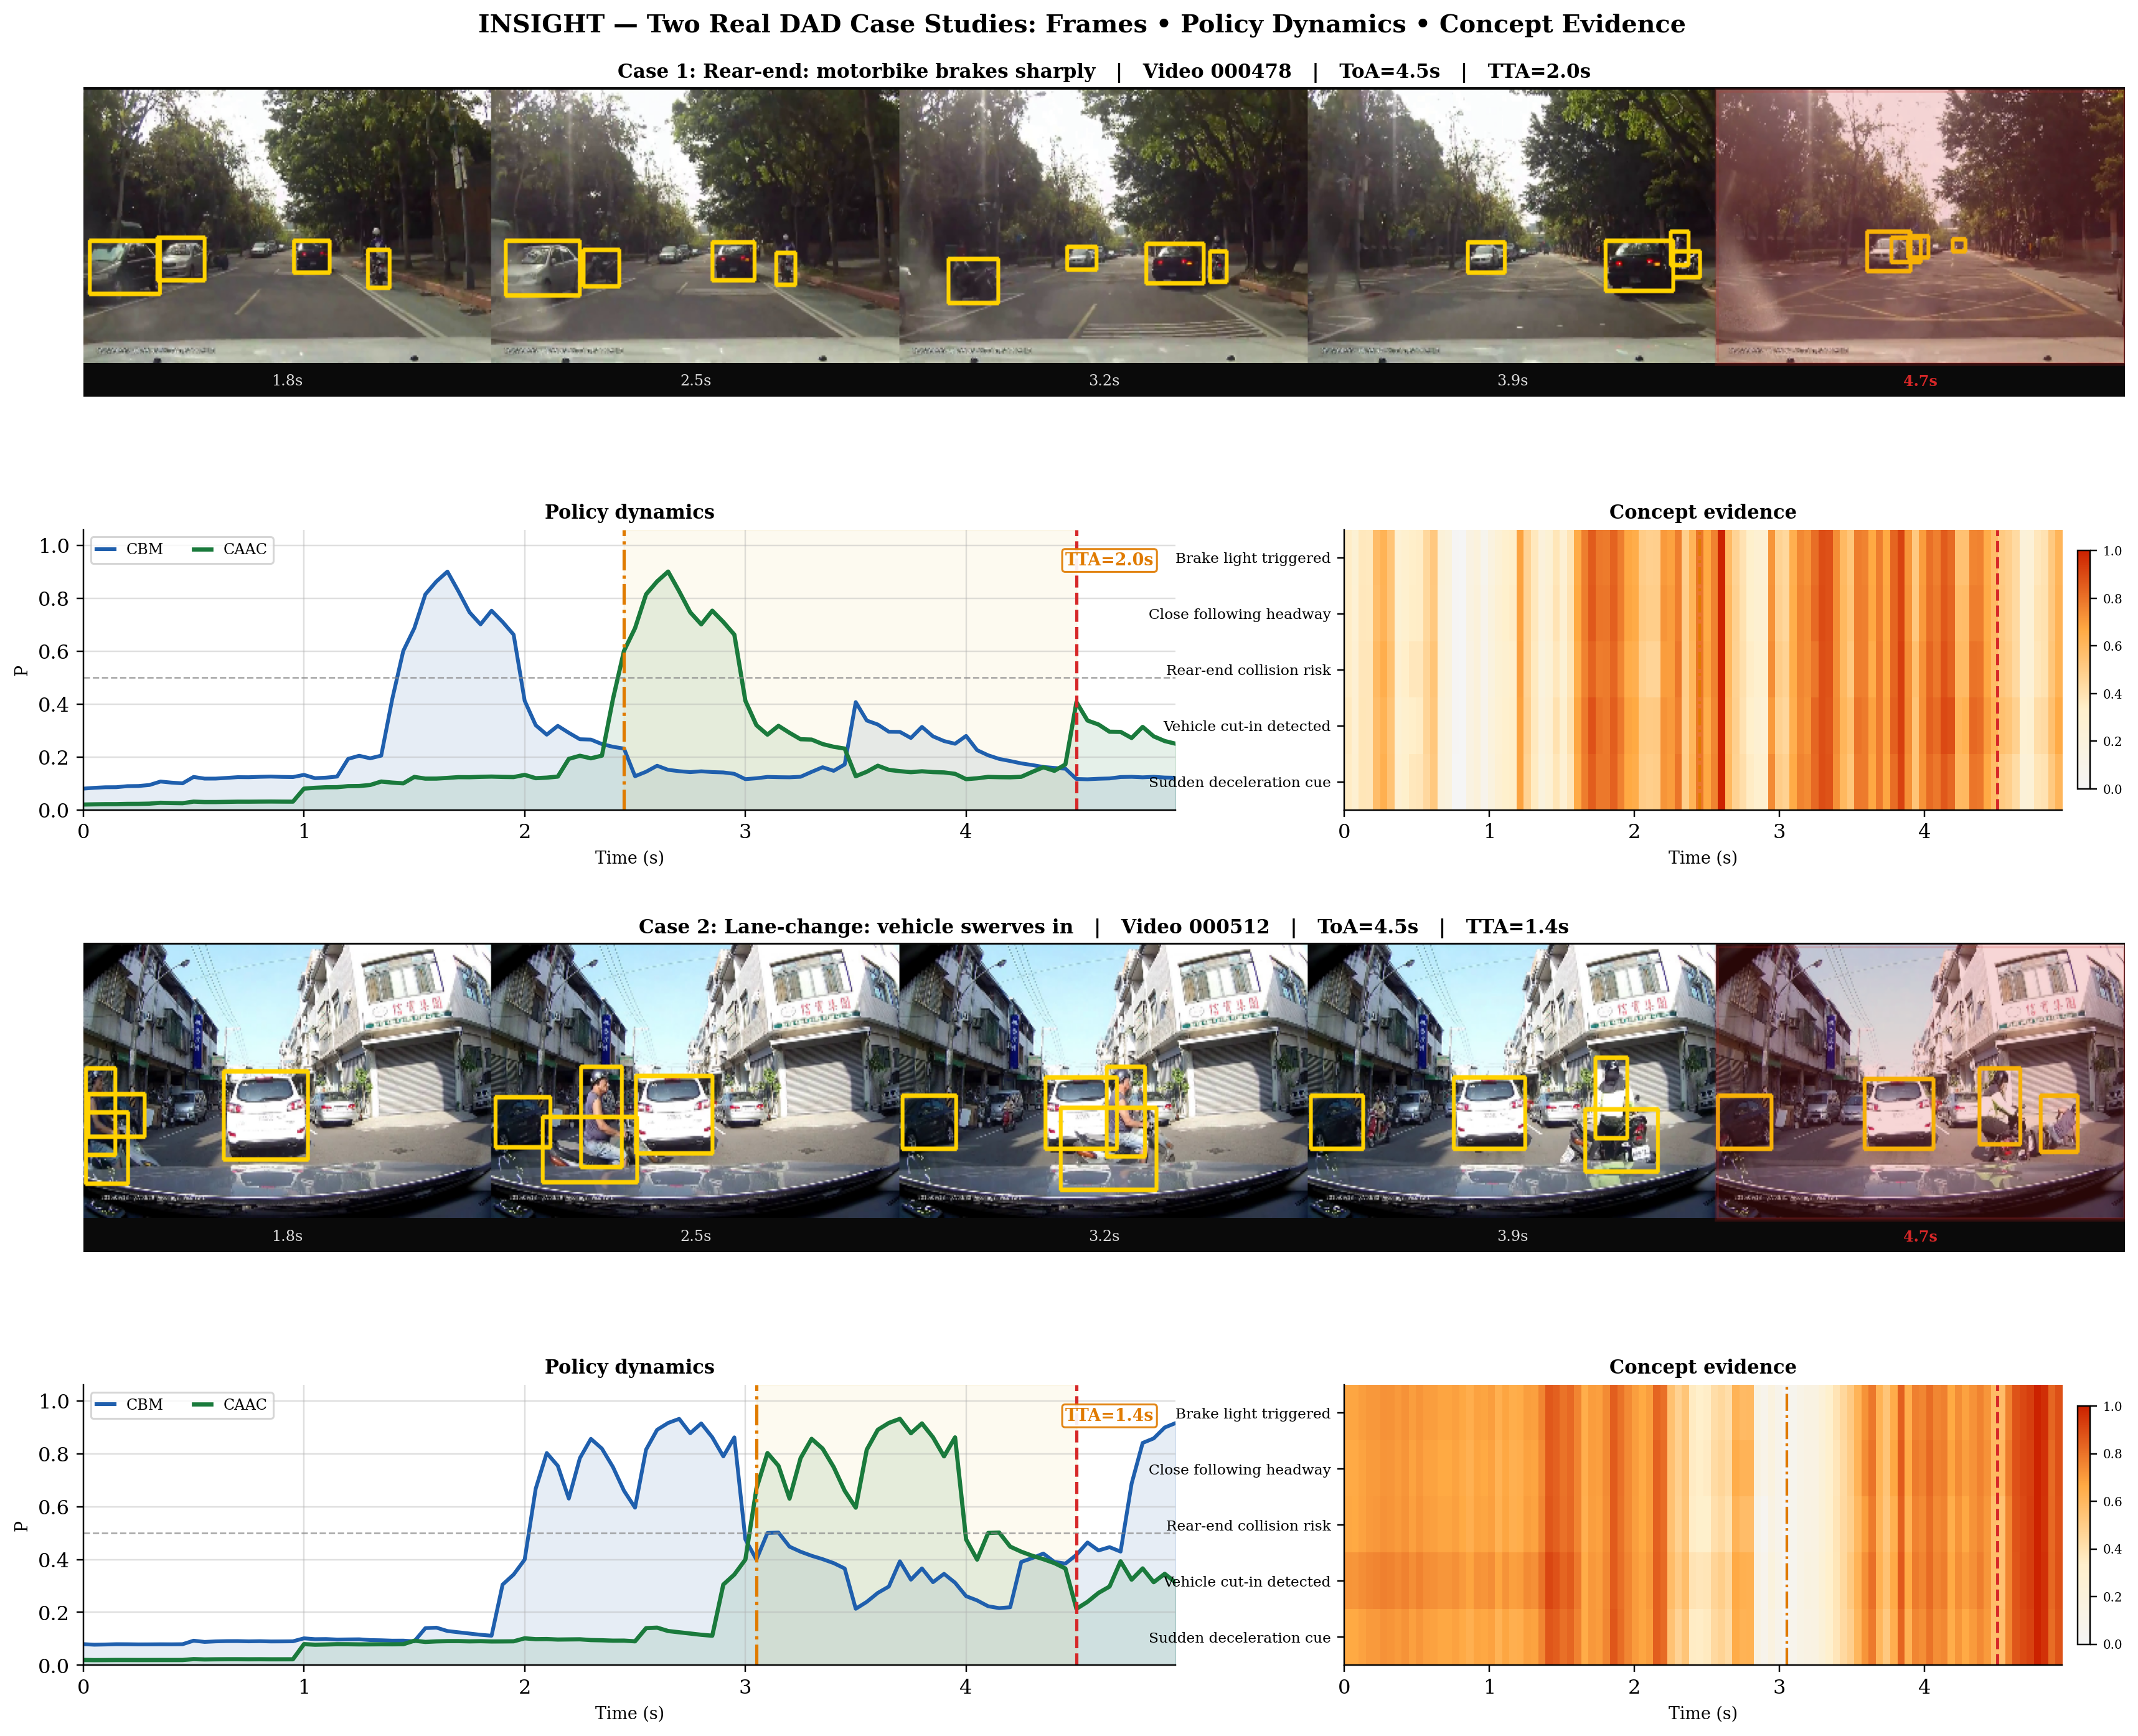
\includegraphics[width=0.985\textwidth]{../figures/insight_fig2_multi_dad_real.png}
  \caption{\textbf{Two-case dual-layer interpretability on real DAD videos.}
  Row pairs show frame strip and policy/concept evidence per case.
  Case diversity spans rear-end and lane-change scenarios.}
  \label{fig:multi}
\end{figure*}

Figures~\ref{fig:interp}--\ref{fig:multi} illustrate the two claims of
\method{} on real DAD scenarios.
The \textbf{WHY layer} surfaces plausible risk concepts before impact;
the \textbf{WHEN layer} converts rising concept trends into earlier alerts;
and the \textbf{CRS ranking} shows that activated concepts form a coherent
scenario-specific safety vocabulary.

\paragraph{Policy-before-peak behaviour.}
A recurring pattern is that the \caac{} curve crosses its alert threshold
\emph{before} the raw accident-probability curve peaks---exactly the
intended behaviour of the time-remaining reward. The policy acts on a
rising semantic trend rather than waiting for maximal confidence.

\paragraph{Frame--concept alignment.}
The strongest visual evidence occurs when a scene change (brake lights,
shrinking headway, lane cut-in) is mirrored by a concept activation spike.
This alignment makes the explanation persuasive and supports careful case
curation: not every high-scoring sample yields equally legible evidence.

\paragraph{Broader case bank.}
Beyond the hero figures, we screened positive DAD test cases ranked by
peak risk, pre-crash area, and rise strength.
The resulting bank spans different traffic geometries and visibility
conditions, reducing cherry-picking risk.

\begin{figure*}[t]
  \centering
  
\includegraphics[width=0.92\textwidth]{../neurips2026/dad_case_contactsheet.png}
  \caption{\textbf{Broader DAD case bank.}
  Positive test cases ranked by peak risk, pre-crash area, and rise
  strength, spanning rear-end, lane-change, and intersection scenarios
  under varied visibility conditions.}
  \label{fig:casebank}
\end{figure*}
